\section{システムの目的}
画像認識による電車の識別をWebアプリケーションとして実装することで,気軽に電車の種類を知ることができるようにすること.
\section{システムの概要}
本システムは,ユーザに画像ないしは動画をブラウザ上で入力してもらい,それをサーバ上で画像認識を用いて処理し,結果をブラウザで表示するWebアプリケーションである.概要図を以下\ref{}に示す.
\begin{figure}
	\label{sys_gaiyou}
	\centering
	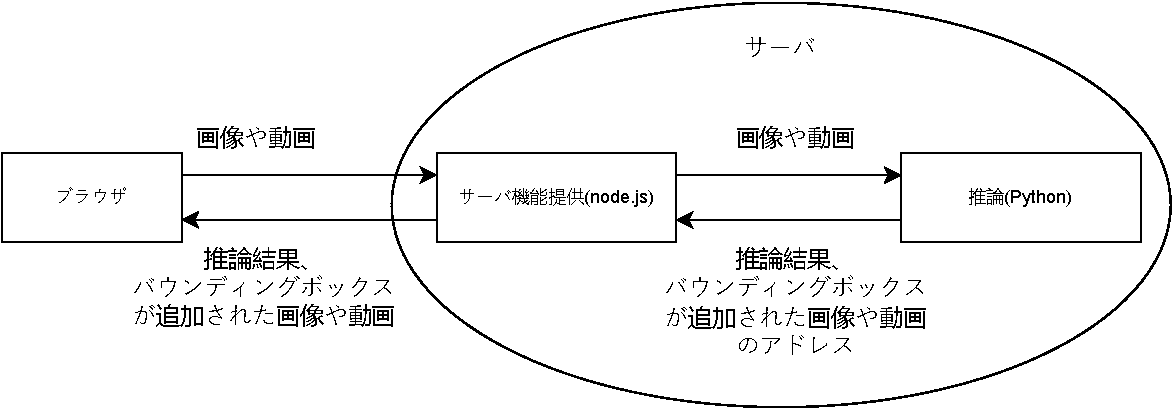
\includegraphics[width=\linewidth]{fig/sys_gaiyou.pdf}
	\figcap{システム概要図}{sys_gaiyou}
\end{figure}

\section{システムの機能}
本システムは,以下の3つの機能を提供する.
\begin{itemize}
\item 電車の画像の分類
\item 電車の画像の識別
\item 電車の動画の識別
\end{itemize}
